%%%%%%%%%%%%%%%%%%%%%%%%%%%%%%%%%%%%%%%%%%%%%%%%%%%%%%%%%%%%%%%%%%%%%%%%%%%%
%% Trim Size: 9.75in x 6.5in
%% Text Area: 8in (include Runningheads) x 5in
%% ws-ijfcs.tex: 05-05-2015
%% Tex file to use with ws-ijfcs.cls written in Latex2E.
%% The content, structure, format and layout of this style file is the
%% property of World Scientific Publishing Co. Pte. Ltd.
%% Copyright 2015 by World Scientific Publishing Co.
%% All rights are reserved.
%%%%%%%%%%%%%%%%%%%%%%%%%%%%%%%%%%%%%%%%%%%%%%%%%%%%%%%%%%%%%%%%%%%%%%%%%%%%
%

\documentclass{ws-ijfcs}
\usepackage{enumerate}
\usepackage{textcomp}
\usepackage{url}
\usepackage{graphicx}
\usepackage[numbers]{natbib}
\usepackage{bussproofs}
\usepackage{tikz}
\usepackage{amssymb}
\usepackage{amsmath}
\usepackage[all,cmtip]{xy}
\usetikzlibrary{positioning, automata}
\usetikzlibrary{decorations.pathmorphing}
 \usetikzlibrary{snakes}


\tikzset{snake it/.style={decorate, decoration=snake}}
\urlstyle{same}
\begin{document}

\markboth{E. Shemetova, A. Okhotin, S. Grigorev}
{The Parallel Complexity of The CFL-Reachability Problem:
Tractable Cases
}

%%%%%%%%%%%%%%%%%%%%% Publisher's Area please ignore %%%%%%%%%%%%%%%
%
\catchline{}{}{}{}{}
%
%%%%%%%%%%%%%%%%%%%%%%%%%%%%%%%%%%%%%%%%%%%%%%%%%%%%%%%%%%%%%%%%%%%%

\title{The Parallel Complexity of CFL-reachability Problem:
Tractable Cases\footnote{
This research was supported by the Russian Science Foundation, grant \textnumero 18-11-00100.}}
%using \LaTeX\footnote{For the title, try not to use more than 3
%lines. Typeset the title in 10 pt Roman, boldface with the first letter of
%important words capitalized.}}%

\author{Ekaterina Shemetova\footnote{
St. Petersburg State University, 
7/9 Universitetskaya nab., Saint Petersburg 199034, Russia.}
\footnote{
St. Petersburg Academic University, 
ul. Khlopina, 8, Saint Petersburg 194021, Russia.}
\footnote{
JetBrains Research,
Primorskiy prospekt 68-70, Building 1, St. Petersburg, 197374, Russia.}
}

\address{
\email{katyacyfra@gmail.com}}

\author{Alexander Okhotin\footnotemark[2] }

\address{
\email{alexander.okhotin@spbu.ru}
}

\author{Semyon Grigorev\footnotemark[2] \footnotemark[4] }

\address{
\email{s.v.grigoriev@spbu.ru}
}


\maketitle

\begin{history}
\received{(Day Month Year)}
%\revised{(Day Month Year)}
\accepted{(Day Month Year)}
%\comby{(xxxxxxxxxx)}
\end{history}

\begin{abstract}
Whereas it has been shown that  the context-free language (CFL) reachability problem is P-complete, there are some subclasses of context-free languages, for which the the CFL-reachability problem lies in NC complexity class. We present two common classes which generalize known examples of such tractable subclasses: bounded-oscillation languages and context-free languages with a poly-slender storage languages. The polynomiality of the rational indices of languages in these classes is proved. Also closure properties of tractable subclasses in terms of the polynomial rational index are investigated.
\end{abstract}

\keywords{CFL-reachability; parallel complexity; digraphs; regular languages; context-free languages; context-free path queries.}

\section{Introduction}
\label{intro}
The context-free language (CFL) reachability problem for a fixed context-free grammar $G$ is stated as follows: given a directed edge-labeled graph $D$ and a pair of nodes  $u$ and $v$, determine whether there is a path from $u$ to $v$ labeled with a string in $L(G)$.  That is, CFL-reachability is a kind of graph reachability problem with path constraints given by context-free languages. It is an important problem underlying some fundamental static code analysis like data flow analysis and program slicing \cite{RepsBasic}, alias analysis \cite*{Chatterjee, alias}, points-to analysis \cite{Incremental} and other \cite{Cai, android, typeflow}, and graph database query evaluation \cite{Azimov, GrigorevRagozina, HellingsCFPQ, RDF}.


Unlike context-free language recognition, which is in NC (when context-free grammar is fixed), the CFL-reachability problem is P-complete \cite{ RepSeq, Yannakakis}. Practically, it means that there is no efficient parallel algorithm for solving this problem (unless P $\neq$ NC). 


While the problem is not parallelizable in general, it is useful to develop more efficient parallel solutions for specific subclasses of the context-free languages. For example, there are context-free languages which admit more efficient parallel algorithms in comparison with the general case of context-free recognition \cite{IBARRA2, IBARRA, Okhotin2014ComplexityOI}.  The same holds for the CFL-reachability problem: there are some examples of context-free languages, for which the CFL-reachability problem lies in NL complexity class (for example, linear and one-counter languages) \cite{labelledGraphs, LReach, Regularrealizability}. 


The CFL-reachability problem has long been known to be P-complete \cite{PCompl}. The parallel complexity of this problem is studied by both static code analysis \cite{RepSeq, RepsBasic} and database communities \cite{ChainQ, Ullman, Yannakakis}. First investigations of this kind were made in terms of Datalog queries, because some classes of Datalog queries (chain queries) can be represented via context-free grammars with the database considered as a graph. 
\begin{example}[Datalog chain query as a context-free grammar]
Consider a database  $D$ with relation ``$child$''. It can also be represented as a digraph $G$, where each node of the graph corresponds to a person, and edges are labeled with a word ``$child$''.


The following Datalog query determines all pairs of people $x$ and $y$ such that $x$ is a descendant of $y$: 


$Desc(x, y)$ :- $Child(x, y)$

$Desc(x, y)$ :- $Child(x, z), Desc(z, y)$


This query can be represented as a context-free grammar with the following rules: 


$Desc \rightarrow Child$ $\vert$ $Child$ $Desc$


$Child  \rightarrow child$


Thus, evaluating the above mentioned Datalog query over database $D$ is equivalent to the solving the CFL-reachability problem for a context-free grammar representation of this query and the edge-labeled graph $G$.
\end{example}
An important undecidability result was obtained by Gaifman et al. \cite{Vardi}:  it is undecidable for a given context-free grammar $G$ whether the CFL-reachability problem for $G$ is in NC or P-complete. However, Ullman and Van Gelder \cite{Ullman} introduce the notion of a \textit{polynomial fringe property} and show that the CFL-reachability problem for context-free grammars having this property is in NC. A context-free grammar $G$ has the \textit{polynomial fringe property} if and only if there is a polynomial $p$ such that, for each regular language $R$ recognized by an automaton with $n$ states, $L(G) \cap R$ is either empty or contains a word shorter than $p(n)$. It is undecidable whether a context-free grammar has the polynomial fringe property. The results of Ullman and Van Gelder \cite{Ullman} can be reinterpreted in terms of the CFL-reachability as follows: 
\begin{enumerate}
\item CFL-reachability for linear languages is in NC, because the corresponding grammars have the polynomial fringe property
\item The same holds for $D_1$ (the Dyck language on one pair of parentheses) and its images under finite-state transductions (one-counter languages)
\item CFL-reachability for $D_2$ (the Dyck language on two pairs of parentheses) is P-complete.
\end{enumerate}
The third result is important because every context-free language can be represented via a regular language and $D_2$ by Chomsky-Sch{\"u}tzenberger theorem, so it is a direct consequence of P-completeness of CFL-reachability problem in general. Also, using the fact that $D_2$ is included in many interesting subclasses of context-free languages, such as visibly pushdown languages \cite{Okhotin2014ComplexityOI}, simple deterministic languages (defined by LL(1) grammars in Greibach normal form), we can state that the CFL-reachability problem for these languages is P-complete. Afrati et al. \cite{ChainQ} investigate the parallel complexity of Datalog simple chain queries and presents the Polynomial Stack Lemma which will be discussed in detail in Section~\ref{sec:poly}. 


The polynomial fringe property is equivalent to having polynomial \textit{rational index}: for a context-free language $L(G)$ having the polynomial rational index is the same as for $G$ to have the polynomial fringe property. More precisely, rational index $\rho_L(n)$ is a function, which denotes the maximum length of the shortest word in $L(G) \cap R$, for arbitrary $R$ recognized by an $n$-state automaton. The notion of a rational index was introduced by L. Boasson et al. \cite{RatBasic} as a complexity measure for context-free languages and was investigated independently of the polynomial fringe property.  In particular, it has been proved that the rational index of $D_1$ is in $O( n^2)$ \cite{Dyck1}. 
Another important result concerns the rational index of languages, which generate all context-free languages (an example of such language is $D_2$). It states that the rational index of such languages is of the order $exp(\Theta(n^2/\ln n))$ \cite{CFRat} and, hence, this is the upper bound on the value of the rational index for every context-free language. An example of a non-generating language with exponential rational index is given in \cite{Regularrealizability}. Also it has been shown that for every algebraic number $\gamma $, a language with the rational index in $\Theta (n^\gamma )$ exists \cite{GreibRat}. 


The CFL-reachability problem is the same as the intersection non-emptiness problem for a context-free language (pushdown automaton) and a regular language (finite automaton), because a labeled graph is a special kind of a nondeterministic finite automaton. The complexity of this problem was studied by Ganardi et al. \cite{ ganardi2016circuit},  Swernofsky et al. \cite{Intersection} and Vyalyi \cite{VyalyiRR}.


The computational complexity of the language reachability for different classes of languages (regular, context-free, context-sensitive) and graphs (acyclic graphs, trees, grid graphs) is discussed in detail by Barret et al. \cite{Barrett}, Holzer et al.\cite{labelledGraphs} and Komarath et al. \cite{LReach}. 


\begin{figure}
\centering
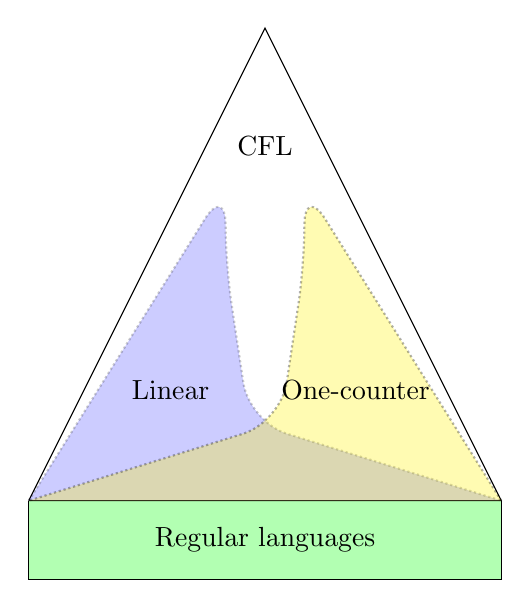
\begin{tikzpicture}
\draw[fill=green, opacity=0.3](0,1) -- (0,0) -- (6,0) --  (6,1);
\draw(0,1) -- (0,0) -- (6,0) --  (6,1);
\draw(0,1) -- (6,1) -- (3, 7) -- (0,1) ;
%\draw[thick, dashed, rounded corners=5mm, fill=yellow, opacity=0.3] (0,1) -- (3.1, 1.5) -- (4.5, 3) -- (6,1);
%\draw[thick, dashed, rounded corners=5mm, fill=red, opacity=0.3] (6,1) -- (2.9, 1.5) -- (1.5, 3) -- (0,1);
\draw[thick, densely dotted, rounded corners=5mm, fill=blue, opacity=0.2](0,1) -- (2.5, 5) -- (2.5,4)-- (2.8, 2) -- (6,1);
\draw[thick, densely dotted, rounded corners=5mm , fill=yellow, opacity=0.3](6,1) -- (3.5, 5) -- (3.5,4)-- (3.2, 2) -- (0,1);
\node (reg) at (3, 0.5) {Regular languages}; 
\node (cfl) at (3, 5.5) {CFL}; 
\node (lin) at (1.8, 2.4) {Linear}; 
\node (one) at (4.15, 2.4) {One-counter}; 
\end{tikzpicture}
\caption{The hierarchy of languages, for which the CFL-reachability problem is in NC.}
\label{hierarchy}      
\end{figure}
Our focus is on investigating the parallel complexity of the CFL-reachability problem. Especially we are interested in generalizing of ``easy'' subclasses and discovering new examples of context-free languages, for which the CFL-reachability problem is in NC. Effective subclasses can be useful in practice, because the general problem is not tractable \cite{ExperimentalCFPQ}. For example, in the case of graph databases, it is important to know the complexity of a given context-free path query. Also it is natural to ask, which properties of subclasses imply that the problem is in NC. Why some languages have polynomial rational indices? What is the difference between them and other subclasses of context-free languages?


The hierarchy of subfamilies of context-free languages, for which the CFL-reachability problem is in NC, is presented in Figure~\ref{hierarchy}. Linear languages and one-counter languages are incomparable families of context-free languages, but both have polynomial rational indices (the polynomial fringe property). These subfamilies have one thing in common: both are defined by strong restrictions on the stack in a pushdown automaton. Our main idea is to generalize the known tractable classes by investigating the restrictions on the PDA store.

\textbf{Our contributions.} Our results can be summarized as follows:
\begin{itemize}
\item We show that the CFL-reachability problem for bounded-oscillation languages of Ganty and Valput \cite{BoundOsc}, is in NC (see Section \ref{sec:osc}). This class generalizes the case of linear languages. 
\item Closure properties of the languages with the polynomial rational indices are investigated in Section \ref{sec:closure}, particularly it is shown that the family of languages with the polynomial rational index is closed under the insertion of a regular language.
\item In Section \ref{sec:poly} we introduce a new subclass of context-free languages: context-free languages with a poly-slender pushdown store languages. These languages are the natural generalization of one-counter languages, and the CFL-reachability problem for them is in NC. Also we show that deciding poly-slenderness of a pushdown store language is in P.
\end{itemize}


\section{Preliminaries}

We introduce !!!!

\subsection{Context-Free Path Querying}

Graph, grammar, etc.

Let $i\pi j$ denote a unique path between nodes $i$ and $j$ of the graph and $l(\pi)$ denotes a unique string which is obtained from the concatenation of edge labels along the path $\pi$.
For a context-free grammar $G = (\Sigma, N, P, S)$ and directed labelled graph $D = (Q, \Sigma, \delta)$, a triple $(A, i, j)$ is \textit{realizable} iff there is a path $i\pi j$ such that nonterminal $A \in N$ derives $l(\pi)$.

\subsection{Tensor-Based algorithm for CFPQ}

\begin{algorithm}[H]
\begin{algorithmic}[1]
\caption{Kronecker product context-free recognizer for graphs}
\label{alg:Kronecker}
\Function{contextFreePathQuerying}{D, G}
\EndFunction
\end{algorithmic}
\end{algorithm}

\subsection{Planar Graphs}

A planar graph $G = (V, E)$ is a graph that can be embedded in the plane.

Outer face - unbounded face in specific embedding.

Directed graph (\textit{digraph})

...

\subsection{Dynamic reachability algorithms}

We consider algorithms that solve the problem of reachability in planar directed graphs. In the \textit{dynamic reachability problem} we are given a graph $G$ subject to edge updates (insertions or deletions) and the goal is to design a data structure that would allow answering queries about the existence of a path.

We need to answer the queries of type: "Is there a directed path from $u$ to $v$ in $G$?". If vertex $u$ in all the queries is fixed we say that algorithm is \textit{single-source}. It is said to be \textit{all-pairs} if vertices $u, v$ can be any vertices of planar digraph $G$, in this case it can be also called \textit{dynamic transitive closure}.

We say that the algorithm is \textit{fully dynamic} if it supports both additions and deletions of edges. It is said to be \textit{semi dynamic} if it supports only one of these updates. If semi dynamic algorithm supports additions only it is called \textit{incremental}, if deletions only - \textit{decremental}.






\section{Bounded-oscillation languages}
\label{sec:osc}
Bounded-oscillation languages were introduced by Ganty and Valput \cite{BoundOsc}. Just like one-counter and linear languages, it is defined by restriction on the pushdown automata. This restriction is based on the notion of \textit{oscillation}, a special measure of how the stack height varies over time. 


Oscillation is defined using a hierarchy of \textit{harmonics}. Let $\bar{a}$ be a \textit{push}-move and $a$ be a \textit{pop}-move. Then a PDA run $r$ can be described by a well-nested sequence $\alpha(r)$ of $\bar{a}$-s and $a$-s. Two positions $i<j$ form a \textit{matching pair} if the corresponding $\bar{a}$ at $i$-th position of the sequence matches with $a$ at $j$-th position. For example, word $\bar{a}\bar{a}\bar{a}aa\bar{a}aa$ has the following set of matching pairs: $\{(1, 8), (2, 5), (3, 4), (6, 7)\}$ ($\bar{a}(\bar{a}(\bar{a}a)a)(\bar{a}a)a$).


Harmonics are inductively defined as follows:
\begin{itemize}
\item  order 0 harmonic $h_0$ is $\varepsilon$
\item  $h_{(i+1)}$ harmonic is $\bar{a}h_ia\ \bar{a}h_ia$.
\end{itemize}
\begin{figure}
\centering
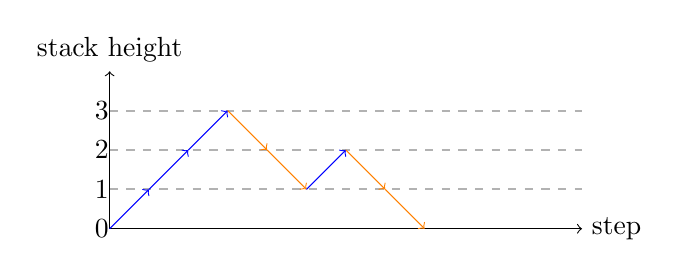
\begin{tikzpicture}
    \draw[thick, dashed, opacity=0.3] (0,0.5) -- (6,0.5);
     \draw[thick, dashed, opacity=0.3] (0,1) -- (6,1);
      \draw[thick, dashed, opacity=0.3] (0,1.5) -- (6,1.5);
      \draw[->] (0,0) -- (6,0) node[right] {step};
      \draw[->] (0,0) -- (0,2) node[above] {stack height};
     \draw[->, blue] (0,0) -- (0.5,0.5);
      \draw[->, blue] (0.5,0.5) -- (1,1);
      \draw[->, blue] (1,1) -- (1.5,1.5);
       \draw[->, orange] (1.5,1.5) -- (2,1);
    \draw[->, orange] (2,1) -- (2.5,0.5);
    \draw[->, blue] (2.5,0.5) -- (3,1);
    \draw[->, orange] (3,1) -- (3.5,0.5);
 \draw[->, orange] (3.5,0.5) -- (4,0);
\node (null) at (-0.1, 0) {0}; 
\node (one) at (-0.1, 0.5) {1}; 
\node (two) at (-0.1, 1) {2}; 
\node (three) at (-0.1, 1.5) {3}; 
    \end{tikzpicture}
\caption{Stack heights during the run of PDA.}
\label{oscb}
\end{figure}


PDA run $r$ is \textit{k-oscillating} if the harmonic of order $k$ is the greatest harmonic that is contained in $r$ after removing $0$ or more matching pairs. \textit{Bounded-oscillation languages} are languages accepted by pushdown automata restricted to $k$-oscillating runs. It is important that the problem whether a given CFL is a bounded-oscillation language is undecidable \cite{BoundOsc}.
\begin{example}
Consider Figure \ref{oscb}. It shows how the stack height changes during the run of a PDA. Corresponding well-nested word $\alpha(r)$ is $\bar{a}\bar{a}\bar{a}aa\bar{a}aa$. The greatest harmonic in this word is order 1 harmonic (moves forming harmonic are marked in bold, removed matching pairs are $(1, 8)$ and $(2, 5)$): $\bar{a}\bar{a}\mathbf{\bar{a}a}a\mathbf{\bar{a}a}a$, therefore oscillation of the run $r$ is 1.
\end{example}


The oscillation of a parse tree of a context-free grammar can be defined similiarly to the oscillation of a PDA run. Given a parse tree $t$, we define corresponding well-nested word $\alpha(t)$ inductively as follows:
\begin{itemize}
\item if $n$ is the root of $t$ then $\alpha(t) = \bar{a}\alpha(n)$
\item if $n$ is a leaf then $\alpha(n)=a$
\item if $n$ has $k$ children then $\alpha(n) = a\underbrace{\bar{a}...\bar{a}}_\text{$k$ times}\alpha(n_1)...\alpha(n_k)$
\end{itemize}


Moreover, given a PDA run $r$, there exists a corresponding parse tree $t$ with the same well-nested word $\alpha(t)=\alpha(r)$ and vice versa \cite{BoundOsc}.


The oscillation of a parse tree is closely related with its $dimension$. For each node $v$ in a tree $t$, its dimension $dim(v)$ is inductively defined as follows:
\begin{itemize}
\item if $v$ is a leaf, then $dim(v)$ = 0
\item if $v$ is an internal node with $k$ children $v_1, v_2, ..., v_k$ for $k \ge 1$, then 
$$
dim(v) = 
 \begin{cases}
   \max_{i \in \{1...k\}}dim(v_i) &\text{if there is a unique maximum}\\
   \max_{i \in \{1...k\}}dim(v_i)+1 &\text{otherwise}
 \end{cases}
$$
\end{itemize}


Dimension of a parse tree $t$ $dim(t)$ is a dimension of its root.  It is observable from the definition that dimension of a tree $t$ is the height of the largest perfect binary tree, which can be obtained from $t$ by contracting edges and accordingly identifying vertices. A tree with dimension $dim(t) = 2$ is illustrated in Figure \ref{oscbtree}.


It is known that the dimension of parse trees and its oscillation are in linear relationship.

\begin{lemma}[\cite{BoundOsc}]
\label{boscdim}
Let a grammar $G = (\Sigma, N, P, S)$ be in Chomsky normal form and let $t$ be a parse tree of $G$. Then $osc(t) - 1 \le dim(t) \le 2osc(t)$.
\end{lemma}

Before we consider the value of the rational index for $k$-bounded-oscillation languages, we need to prove the following.
\begin{figure}
\centering
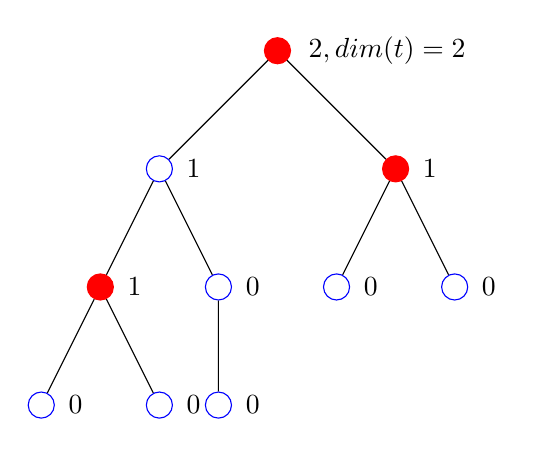
\begin{tikzpicture}[
level 1/.style={sibling distance=3cm},
level 2/.style={sibling distance=1.5cm}]
%\tikzstyle{every node}=[circle,draw]

\node[circle,draw] (Root) [ fill=red, red] {}
    child {
    node[circle,draw, blue] (l) {} 
    child { node[circle,draw, fill=red, red](ll) {}
            child { node[circle,draw, blue] (p) {} }
            child { node[circle,draw, blue] (pl) {} }
             }
    child { node[circle,draw, blue](lr) {} 
          child { node[circle,draw, blue] (plr) {} }
      }
}
child {
    node[circle,draw,  fill=red, red] (r) {}
    child { node[circle,draw, blue] (rl) {}} 
    child { node[circle,draw, blue] (rr) {} }
};
\node  [right=0.05cm of p] {0};
\node  [right=0.1cm of Root] {$2, dim(t)=2$};
\node  [right=0.05cm of l] {1};
\node  [right=0.05cm of r] {1};
\node  [right=0.05cm of ll] {1};
\node  [right=0.05cm of lr] {0};
\node  [right=0.05cm of pl] {0};
\node  [right=0.05cm of plr] {0};
\node  [right=0.05cm of rl] {0};
\node  [right=0.05cm of rr] {0};
\end{tikzpicture}
\caption{A tree $t$ with $dim(t)=2$. Nodes having children without unique maximum are filled.}
\label{oscbtree}            
\end{figure}
\begin{lemma}
\label{lem:treeheight}
Let  $G = (\Sigma, N, P)$ be a context-free grammar,  $D=(V, E, \Sigma)$ be a directed labeled graph with $n$ nodes. Let $w$ be the shortest string in $L(G)\cap L(D)$. Then the height of every parse tree for $w$ does not exceed $|N|n^2$.
\end{lemma}

\begin{proof}
Consider a parse tree for $w$ which is constructed in the following way: every node of the parse tree is marked with realizable triple (see Definition~\ref{def:triple}); for every rule $A \rightarrow A_1A_2...A_k \in P$ a node labeled with $(A, i, j)$ has children marked with $(A_1, i, v_1), (A_2, v_1, v_2), ..., (A_k, v_k, j)$, and every leaf is marked with a triple $(a, i, j)$, where $(i, j)$ is an edge of the input graph labeled with a symbol $a$. Assume that such parse tree for $w$ has a height of more than $|N|n^2$. Consider a path from the root of the parse tree to a leaf, which has the length of more than $|N|n^2$. There are $|N|n^2$ unique labels $(A, i, j)$ for nodes of the parse tree, so according to the pigeonhole principle, this path has at least two nodes with the same label. This means that the parse tree for $w$ contains at least one subtree $t$ with label $(A, i, j)$ at the root, which has a subtree $t'$ with the same label. Then we can change $t$ with $t'$ and get a new string $w'$ which is shorter than $w$. But $w$ is the shortest, then we have a contradiction.

\end{proof}
From Lemma \ref{lem:treeheight} we have that rational index of linear languages is in $O(n^2)$. 
\begin{lemma}
\label{oscbnddim}
Let $G$ be a grammar $G = (\Sigma, N, P, S)$ in Chomsky normal form, such that every parse tree $t$ has $dim(t) \le d$, where $d$ is some constant. Let $D=(V, E, \Sigma)$ be a directed labeled graph with $n$ nodes. Then $\rho_{L(G)}$ is in $O({(|N|n^2)}^d)$ in the worst case.
\end{lemma}
\begin{proof}
Proof by induction on dimension $dim(t)$.
\\
\textbf{Basis.} $dim(t) = 1$.
\\
Consider a tree $t$ with the dimension $dim(t) = 1$. The root of the tree has the same dimension and has two children (because the grammar is in Chomsky normal form). There are two cases:  first, when both of child nodes have dimension equal to 0, then the tree has only two leaves, and second, when one of the children has dimension 1, and the second child has dimension 0. For the second case we can recursively construct a tree with the maximum number of leaves in the following way. Every internal node of such a tree has two children, one of which has dimension equal to 0 and therefore has only one leaf. By Lemma \ref{lem:treeheight}, the maximum height $h$ of such tree is at most $|N|n^2$, so the number of leaves in it is $O(h) = O(|N|n^2)$.
\\
\textbf{Inductive step.} $dim(t) = d + 1$.
\\
Assume that $\rho_{L(G)}$ is at most $O(h^{d})$ for every $d$ in the worst case, where $h$ is the height of the tree. We have two cases for the root node with dimension equal to $d+1$: 1) both of children have a dimension equal to $d$, then by proposition the tree of heght $h$ has no more than $O(h^{d})$ leaves; 2) one of the children has a dimension $d + 1$, and the second child $v$ has a dimension $dim(v) \le d$. Again, a tree with the maximum number of leaves can be constructed recursively:  each node of such tree has two children $u$ and $v$ with dimensions $d+1$ and $d$ respectively (the greater the dimension of the node, the more leaves are in the corresponding tree in the worst case). By the induction assumption there are no more than $(h-1)^d + (h-2)^d + (h-3)^d + ... + 1 = O(h^{d+1})$ leaves, so the claim holds for $dim = d+1$. Finally, $\rho_{L(G)}$ is almost $O(h^{d}) = O({(|N|n^2)}^d)$ for every $d$, because $h \le |N|n^2$ by Lemma \ref{lem:treeheight}. 
\end{proof}
Combining Lemma \ref{boscdim} and Lemma \ref{oscbnddim}, we can deduce the following.
\begin{theorem}
\label{oscbndosc}
Let $L$ be a $k$-bounded-oscillation language with grammar $G = (\Sigma, N, P, S)$ in Chomsky normal form and $D=(V, E, \Sigma)$ be a directed labeled graph with $n$ nodes. Then $\rho_{L(G)}$ is in $O({|N|}^{2k}n^{4k})$ in the worst case.
\end{theorem}
\begin{proof}
By Lemma~\ref{boscdim}, every parse tree of bounded-oscillation language has also bounded dimension. Then the maximum value of the dimension of every parse tree of $k$-bounded-oscillation language is $2k$. By Lemma~\ref{oscbnddim}, $\rho_{L(G)}$ is in $O({(|N|n^2)}^d)$ and, thus, $\rho_{L(G)}$ does not exceed $O({(|N|n^2)}^{2k}) = O({|N|}^{2k}n^{4k})$.
\end{proof}

As we can see from the proof of Lemma~\ref{oscbnddim}, the family of linear languages is included in the family of bounded-oscillation languages. The reason is that the family of bounded-oscillation languages generalizes the family of languages accepted by finite-turn pushdown automata \cite{BoundOsc}. It is interesting that for general PDA, particularly for $D_2$, the value of osciillation is not constant-bounded: it depends on the length of input and does not exeed $O(\log n)$ for the input of length $n$ \cite*{Gundermann, Wechsung}. However, for some previously studied subclasses of context-free languages,  oscillation is bounded by a constant.

\begin{example}[Superlinear languages \cite{superlinear}] A context-free grammar $G = (\Sigma, N, P, S)$ is \textit{superlinear} if all productions of $P$ satisfy these conditions:
\begin{enumerate}
\item there is a subset $N_L \subseteq N$ such that every $A \in N_L$ has only linear productions $A\rightarrow aB$ or $A\rightarrow Ba$, where $B \in N_L$ and $a \in \Sigma$.
\item if $A \in N \setminus N_L$, then $A$ can have non-linear productions of the form $A \rightarrow BC$ where $B\in N_L$ and $C \in N$, or linear productions of the form $A\rightarrow \alpha B$ $\vert$ $B \alpha$ $\vert$ $\alpha$ for $B \in N_L$, $\alpha \in \Sigma^*$.
\end{enumerate}
From the grammar $G$ it is observable that its parse trees have dimension at most 2. From 
Lemma~\ref{oscbnddim}, if dimensions of all parse trees are bounded by some $k$ then the rational index of such language is polynomial, so the CFL-reachability problem for superlinear languages is in NC. 
\end{example}
\section{Closure properties of languages with polynomial rational indices}
\label{sec:closure}
Given a context-free language $L$ with the polynomial rational index, it is interesting to find which language operations preserve this property.  Boasson et al. \cite{RatBasic} give the following useful relations for polynomial indices of two languages $L$ and $L'$.
\begin{lemma}[\cite{RatBasic}]
\label{lem:closure}
Context-free languages with polynomial rational indices are closed under intersection with a regular language, union, concatenation, the Kleene star, homomorphism and inverse homomorphism. More precisely,
\begin{itemize}
\item $\rho_{L \cup L'}(n) \le  \max{(\rho_L(n), \rho_{L'}(n))} $
\item $\rho_{LL'}(n) \le \rho_L(n) + \rho_{L'}(n)$
\item $\rho_{L^{*}}(n) \le n(\rho_L(n))$
\item $\rho_{L \cap R}(n) \le \rho_L(nm)$, where $R$ is a regular language recognised by an $m$-state automaton
\item $\rho_{h(L)}(n) \le \rho_L(n)$ and $\rho_{h^{-1}(L)}(n) < n(\rho_L(n) +1)$, where $h: \Sigma^* \rightarrow \Delta^*$ is a homomorphism
\item $\rho_{\tau(L)}(n) \le (mn + 1)\rho_L(mn)$, where $\tau$ is a rational transduction and $m$ is some integer.
\end{itemize}
\end{lemma}
 From the relations above it is easy to see that the family of context-free languages with polynomial rational indices is a full trio. Every full trio is closed under left and right quotient with regular languages, prefix, suffix, infix, and outfix \cite{GinsburgAlgebraic}. Obviously, CFLs with the polynomial rational indices languages are closed under reversal.  Next we show that context-free languages with the polynomial rational indices are closed under insertion of a regular language.
\begin{theorem}
Context-free languages with the polynomial rational indices are closed under the insertion of a regular language. 
\\Particularly, $\rho_{L_{INSERT(K)}}(n) \le (mn + 1)\rho_L(mn)$, where $m$ is the number of states in the NFA accepting $K$.
\end{theorem}
\begin{proof}
 Let $L$ be a language with the polynomial rational index over an alphabet $\Sigma$ and $K$ be a regular language over an alphabet $\Delta$, where an NFA $M(K)$ with $m$ states is an NFA accepting $K$.  Define a homomorphism $h: \Delta^*  \rightarrow \bar{\Delta}^{*}$, such that $h(a)=\bar{a}$,  $\forall a \in \Delta$. In simple words, $h$ makes all symbols from $\Delta$ ``marked''. Then, by defining a homomorphism $g$, such that $g(a) = \varepsilon$, $\forall a \in \bar{\Delta}$ ($g$ erases the symbols of $\bar{\Delta}$), one can insert an arbitrary number of symbols from $\bar{\Delta}$ into strings in $L$ using an inverse homomorphism $g^{-1}$. To obtain a string from $L_{INSERT(K)}$ it is left to intersect $g^{-1}(L)$ with a regular set $K'$ containing strings in the form $xyz$, where $x, z \subseteq \Sigma^{*}$ and $y \in h(K)$. Then ``marked'' symbols from  $\bar{\Delta}$ is unmarked by a homomorphism $\phi:  \bar{\Delta^*}  \rightarrow \Delta^{*}$, where $\phi(\bar{a}) = a$, $\forall \bar{a} \in \bar{\Delta}$. Finally, every word $w' \in L_{INSERT(K)}$ can be written as $\phi(g^{-1}(w) \cap K') = \tau(w)$, where $w \in L$ and $\tau$ is a rational transduction. By Lemma~\ref{lem:closure}, languages with the polynomial rational indices are closed under rational trunsductions, so $L_{INSERT(K)}$ has the polynomial rational index. An NFA $M(K')$ can be easily constructed from $M(K)$ and has $O(m)$ states. Then the value of the rational index $\rho_{L_{INSERT(K)}}(n) \le (mn + 1)\rho_L(mn)$.
\end{proof}



Using closure properties, it is easier to find new subclasses of context-free languages for which the CFL-reachability problem is in NC.
\begin{example}[Metalinear languages \cite{metalinear}.]
Let $G = (\Sigma, N, P, S)$ be a context-free grammar. $G$ is \textit{metalinear} if all productions of $P$ are of the following forms:
\begin{enumerate}
\item $S \rightarrow A_1A_2...A_k$, where $A_i \in N \setminus \{S\}$
\item $A \rightarrow u$, where $A \in N \setminus \{S\}$ and $u \in (\Sigma^*((N \setminus \{S\}) \cup {\varepsilon})\Sigma^*)$
\end{enumerate}


The width of a metalinear grammar is $max\{k\vert S \rightarrow A_1A_2...A_k \}$. Metalinear languages of width 1 are obviously linear languages. It is easy to see that every metalinear language is a union of concatenations of $k$ linear languages. Linear languages have polynomial rational index,  CFLs with the polynomial rational index are closed under concatenation and union, so metalinear languages have the polynomial rational index and, hence, is in NC.
\end{example}


\section{Languages with poly-slender store languages}
\label{sec:poly}
In the Section~\ref{sec:osc} restriction on PDA in terms of variability of stack height was described. This restriction does not hold for PDA for the language $D_1$; however this language has polynomial rational index. In this section, another kind of stack restriction is considered~--- poly-slenderness of a pushdown store language as a measure of how stack contents vary along accepting computations of PDA.


For a PDA $M$, its \textit{pushdown store language} $P(M)$ consists of all words
occurring on the stack in accepting computations of $M$. It is well-known that the store language of every PDA is regular. The language $D_1$ is a one-counter language, so its pushdown store language is $Z^*Z_0$, where $Z$ is a single pushdown symbol and $Z_0$ is the bottom symbol.


Afrati et al. \cite{ChainQ} define the notion of \textit{polynomial stack property} and show that if a PDA has the polynomial stack property, then the corresponding query has the polynomial fringe property (and hence, lies in NC). A PDA $M$ has the polynomial stack property if and only if the number of different strings of length $k$ occuring in the stack in any accepting computation of $M$ is bounded by $O(k^d)$,  for $d \ge 0$. For example, the usual PDA for $D_1$ has the polynomial stack property, because there is only one possible variant of contents for every stack height. 


Generalizing an example of the family of one-counter languages, we can define the family of languages whose PDAs have the polynomial stack property~--- languages with a \textit{poly-slender} pushdown store language (or storage language with the polynomial density). The density of a language is a function $f(n)$ that shows the number of words of length $n$ in the language. A language $L \subseteq \Sigma^*$ is called \textit{poly-slender language (or with the polynomial density)} if the function $f(n)$ is bounded by $O(n^k)$ for some $k \ge 0$. For example, the language $Z^*Z_0$ is of polynomial density (even of a constant density), whereas the language ${(Z_1 + Z_2)}^*Z_0$ is of exponential density.


Whereas the polynomial fringe property of a query is undecidable \cite{Ullman}, it is decidable in polynomial time whether a given PDA has a poly-slender storage language. At first, for a given NFA it is decidable whether its language has a polynomial or exponential density \cite*{sparseness, poldens}. Gawrychowski et al. \cite{Gawrychowski} give an algorithm for testing whether $L(M)$ is of polynomial or exponential density in $O(|Q| + |\delta|)$ time for an NFA $M = (Q,\Sigma,\delta ,q_{0},F)$. An NFA for pushdown store language of a given PDA $\mathcal{A} = (Q', \Sigma', \Gamma, \delta', q_0', Z_0, F')$ can be constructed directly in $O({|Q'|}^5{|\Gamma|}^2|\delta'|)$ time \cite{PSLDirect}. This construction uses the notion of meaningful triples, which form the states of NFA. A triple $[p, Z, q] \in Q' \times \Gamma \times Q'$ is \textit{meaningful} if there exists a computation of $\mathcal{A}$ starting from state $p$ with the sole symbol $Z$ in the pushdown, and ending in $q$ with the empty pushdown. By definition, there are at most $|\Gamma|{|Q'|}^2$ meaningful triples, and, hence, states of NFA. 



\section{Conclusions and open problems}
\label{sec:conc}
\begin{figure}
\centering
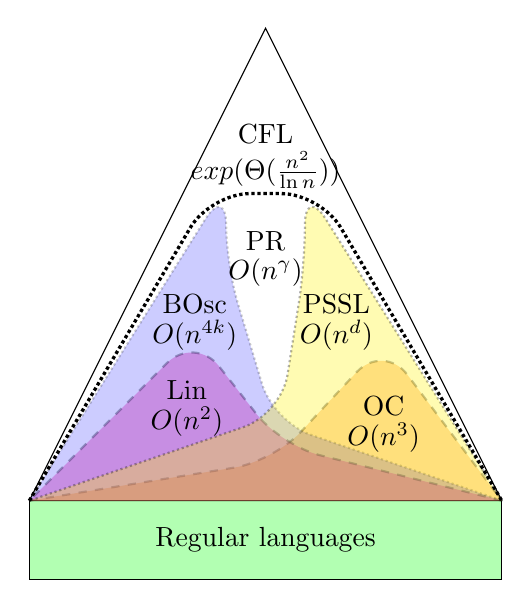
\begin{tikzpicture}
\draw[fill=green, opacity=0.3](0,1) -- (0,0) -- (6,0) --  (6,1);
\draw(0,1) -- (0,0) -- (6,0) --  (6,1);
\draw(0,1) -- (6,1) -- (3, 7) -- (0,1) ;
\draw[thick, dashed, rounded corners=5mm, fill=orange, opacity=0.3] (0,1) -- (3.1, 1.5) -- (4.5, 3) -- (6,1);
\draw[thick, dashed, rounded corners=5mm, fill=magenta, opacity=0.3] (6,1) -- (3.2, 1.7) -- (2.1, 3.1) -- (0,1);
\draw[thick, densely dotted, rounded corners=5mm, fill=blue, opacity=0.2](0,1) -- (2.5, 5) -- (2.5,4)-- (3.1, 2) -- (6,1);
\draw[thick, densely dotted, rounded corners=5mm , fill=yellow, opacity=0.3](6,1) -- (3.5, 5) -- (3.5,4)-- (3.2, 2.1) -- (0,1);
%\draw[thick, dashed, rounded corners=5mm, fill=red, opacity=0.3] (0,1) -- (2.3, 2.4)  -- (3.3, 1.1) -- (6,1);
\draw[very thick, densely dotted, rounded corners=5mm] (0,1) -- (2.3, 4.9) -- (3.7, 4.9) -- (6,1);
\node (reg) at (3, 0.5) {Regular languages}; 
\node (cfl) at (3, 5.65) {CFL}; 
\node (pr) at (3, 4.3) {PR};
\node (prrho) at (3, 3.9) {$O(n^\gamma)$};
\node (cflrho) at (3, 5.2) {$exp(\Theta(\frac{n^2}{\ln n}))$}; 
\node (plin) at (2, 2.4) {Lin}; 
%\node (lin) at (2.1, 1.5) {Lin}; 
\node (osc) at (2.1, 3.5) {BOsc}; 
\node (one) at (4.5, 1.8) {$O(n^3)$}; 
\node (onerho) at (4.5, 2.2) {OC}; 
\node (pssl) at (3.9,3.5) {PSSL}; 
\node (psslrho) at (3.9,3.1) {$O(n^{d})$}; 
%\node (linrho) at (2, 1.2) {$O(n^2)$}; 
\node (linrho) at (2, 2) {$O(n^2)$}; 
\node (oscrho) at (2.1, 3.1) {$O(n^{4k})$}; 
\end{tikzpicture}
\caption{The hierarchy of languages with polynomial rational indices and corresponding upper bounds on the value of rational index. PR~--- the family of CFLs with the polynomial rational indices, BOsc~--- bounded-oscillation languages, PSSL~--- CFLs with poly-slender storage languages, OC~--- one-counter languages, Lin~--- linear languages, $n$~--- number of vertices in graph (NFA), $|N|$~--- the number of non-terminals of grammar in Chomsky normal form, $k$~--- the oscillation value, $d$~--- the degree of polynomial density of the pushdown storage language, $\gamma$~--- algebraic number.}
\label{hierarchyfinal}      
\end{figure}
We have obtained two classes, which extend the classes in the recent literature \cite{ChainQ, labelledGraphs, LReach, Regularrealizability, Ullman}, for which the CFL-reachability problem is in NC. One of them is the class of bounded-oscillation languages, which generalizes the linear languages. The second class is context-free languages with a poly-slender pushdown store languages, which is the generalization of the one-counter languages. Recall that regular languages have the polynomial fringe property (and are accepted by a PDA with a bounded stack height), also it is known that L-reachability for regular languages is in NL \cite{LReach, Yannakakis}. Thereby it has been demonstrated that some natural restrictions on the pushdown storage implies the polynomial rational index for the corresponding context-free languages: the low variability of stack height during the PDA run (bounded-oscillation PDA) and the limited number of possible stack contents (languages with poly-slender pushdown store languages). The updated hierarchy of tractable subclasses and corresponding upper bounds on the rational indices are illustrated in Figure~\ref{hierarchyfinal}.


It will be interesting to know whether there is any other stack restriction which implies polynomial rational index. Are there any other properties (except polynomial rational index) which make the CFL-reachability problem solvable in NC? For example, there is a Datalog query, which does not have the polynomial fringe property but its evaluation is in NC \cite{Kanellakis}. One can also approach this question from another direction by looking for simple subfamilies of context-free languages that would have P-complete CFL-reachability problem.


Also it is interesting to consider other machine models with stores having store restrictions examined in this work. Do these restrictions imply that certain properties could become decidable or their complexity could be reduced? Store languages of different machine models and their applications are studied in \cite{ Ibarra2018OnSL, IBARRA201928}.


We considered the CFL-reachability problem for a fixed context-free languages and arbitrary graphs. What tractable cases can be obtained for a fixed graphs and an arbitrary context-free language? The known and trivial examples are acyclic graphs and trees. Can we have more complicated classes of graphs for which the CFL-reachability problem is in NC? Interesting algebraic properties of such graphs (NFA) are given in \cite{ganardi2016circuit}, but automata-theoretic characterizations of these properties remain to be found.


%%For cite command type as \cite{1}; \cite{3,6} and \cite{2,4,6}.
%%For refcite command type as Refs.~[\refcite{1}];
%%[\refcite{1},\refcite{3}] and [\refcite{1}--\refcite{4}].


\section*{Acknowledgments}
This research was supported by the Russian Science Foundation, grant \textnumero 18-11-00100.



\bibliographystyle{ws-ijfcs}  
\bibliography{paper}
\end{document}